%%%%%%%%%%%%%%%%%%%%%%%%%%%%%%%%%%%%%%%%%
% Beamer Presentation
% LaTeX Template
% Version 1.0 (10/11/12)
%
% This template has been downloaded from:
% http://www.LaTeXTemplates.com
%
% License:
% CC BY-NC-SA 3.0 (http://creativecommons.org/licenses/by-nc-sa/3.0/)
%
%%%%%%%%%%%%%%%%%%%%%%%%%%%%%%%%%%%%%%%%%

%------------------------------------------------------------------------------------------------
%   PACKAGES AND THEMES
%------------------------------------------------------------------------------------------------

\documentclass[table, xcolor = {dvipsnames}, 9pt]{beamer}
\usepackage{tikz}
\usetikzlibrary{backgrounds}
\usetikzlibrary{arrows,shapes}
\usetikzlibrary{tikzmark}
\usetikzlibrary{calc}
\usetikzlibrary{colorbrewer}
\mode<presentation> {

% The Beamer class comes with a number of default slide themes
% which change the colors and layouts of slides. Below this is a list
% of all the themes, uncomment each in turn to see what they look like.

\usetheme{default}
%\usetheme{AnnArbor}
%\usetheme{Antibes}
%\usetheme{Bergen}
%\usetheme{Berkeley}
%\usetheme{Berlin}
%\usetheme{Boadilla}
%\usetheme{CambridgeUS}
%\usetheme{Copenhagen}
%\usetheme{Darmstadt}
%\usetheme{Dresden}
%\usetheme{Frankfurt}
%\usetheme{Goettingen}
%\usetheme{Hannover}
%\usetheme{Ilmenau}
%\usetheme{JuanLesPins}
%\usetheme{Luebeck}
%\usetheme{Madrid}
\usetheme{metropolis}
%\usetheme{Malmoe}
%\usetheme{Marburg}
%\usetheme{Montpellier}
%\usetheme{PaloAlto}
%\usetheme{Pittsburgh}
%\usetheme{Rochester}
%\usetheme{Singapore}
%\usetheme{Szeged}
%\usetheme{Warsaw}

% As well as themes, the Beamer class has a number of color themes
% for any slide theme. Uncomment each of these in turn to see how it
% changes the colors of your current slide theme.

%\usecolortheme{albatross}
%\usecolortheme{beaver}
%\usecolortheme{beetle}
%\usecolortheme{crane}
%\usecolortheme{dolphin}
%\usecolortheme{dove}
%\usecolortheme{fly}
%\usecolortheme{lily}
%\usecolortheme{orchid}
%\usecolortheme{rose}
\usecolortheme{seagull}
%\usecolortheme{seahorse}
%\usecolortheme{whale}
%\usecolortheme{wolverine}
\usefonttheme{professionalfonts}
%\setbeamertemplate{footline} % To remove the footer line in all slides uncomment this line
%\setbeamertemplate{footline}[page number] % To replace the footer line in all slides with a simple slide count uncomment this line

%\setbeamertemplate{navigation symbols}{} % To remove the navigation symbols from the bottom of all slides uncomment this line
}

\usepackage{graphicx} % Allows including images
\usepackage{booktabs} % Allows the use of \toprule, \midrule and \bottomrule in tables
\usepackage{multirow}
\usepackage{xspace}
\usepackage{natbib}
\usepackage{hyperref}
\usepackage{diagbox}
\usepackage{makecell}
\usepackage{xparse}
\usepackage{subfig}
\usepackage{amsfonts,amsthm,amsmath,amssymb}
\usepackage{mathtools, nccmath}
\usepackage[ruled, vlined, linesnumbered]{algorithm2e}
\usepackage{wrapfig}
\usepackage{comment}  
\usepackage{bbm}
\usepackage{bm}
\usepackage{empheq}
\usepackage{pgfplots}
\usepgfplotslibrary{colorbrewer}
\usepackage{animate}
\usepackage{array}
\usepackage{ragged2e}
\newcolumntype{P}[1]{>{\RaggedRight\hspace{0pt}}p{#1}}
\newcolumntype{X}[1]{>{\RaggedRight\hspace*{0pt}}p{#1}}

% color box
\usepackage{tcolorbox}
\usepackage{tikz}
\usetikzlibrary{backgrounds}
\usetikzlibrary{arrows,shapes}
\usetikzlibrary{tikzmark}
\usetikzlibrary{calc}
% Commands for Highlighting text -- non tikz method
\newcommand{\highlight}[2]{\colorbox{#1!17}{$\displaystyle #2$}}
%\newcommand{\highlight}[2]{\colorbox{#1!17}{$#2$}}
\newcommand{\highlightdark}[2]{\colorbox{#1!47}{$\displaystyle #2$}}

% my custom colors for shading
\colorlet{mhpurple}{Plum!80}


% Commands for Highlighting text -- non tikz method
\renewcommand{\highlight}[2]{\colorbox{#1!17}{#2}}
\renewcommand{\highlightdark}[2]{\colorbox{#1!47}{#2}}

\usepgfplotslibrary{colorbrewer}

\newcommand\mybox[2][]{\tikz[overlay]\node[fill=lightgray,inner sep=2pt, anchor=text, rectangle, rounded corners=1mm,#1] {#2};\phantom{#2}}
\hypersetup{unicode=true,
            bookmarksnumbered=true,
            bookmarksopen=true,
            bookmarksopenlevel=2,
            breaklinks=false,
            pdfborder={0 0 1},
            hypertexnames=false,
            pdfstartview={XYZ null null 1}}
\usepackage{xcolor}
\hypersetup{
    colorlinks,
    linkcolor={red!50!black},
    citecolor={blue!50!black},
    urlcolor={blue!80!black}
}
\newcommand\myheading[1]{%
  \par\bigskip
  {\Large\bfseries#1}\par\smallskip}
\newcommand\given[1][]{\:#1\vert\:}
\theoremstyle{plain}
\newtheorem{thm}{Theorem}
\newtheorem{prop}{Proposition\thisthmnumber}
\newtheorem{lem}{Lemma\thisthmnumber}
\newtheorem{cor}{Corollary}
\newtheorem{defin}{Definition}
\newtheorem{algo}{Algorithm}
\newcommand*\diff{\mathop{}\!\mathrm{d}}
\newcommand*\Diff[1]{\mathop{}\!\mathrm{d^#1}}
\newcommand{\thisthmnumber}{}
\newcommand*{\QEDA}{\hfill\ensuremath{\blacksquare}}%
\newcommand*{\QEDB}{\hfill\ensuremath{\square}}%
\newcommand{\norm}[1]{\left\lVert#1\right\rVert}
\DeclareMathOperator{\N}{\mathbb{N}}
\DeclareMathOperator{\E}{\rm{E}}
\DeclareMathOperator{\R}{\mathbb{R}}
\DeclareMathOperator{\Var}{\rm{Var}}
\DeclareMathOperator{\Cov}{\rm{Cov}}
\DeclareMathOperator{\e}{\rm{e}}
\DeclareMathOperator{\logit}{\rm{logit}}
\DeclareMathOperator{\indep}{{\perp\!\!\!\perp}}
\DeclareMathOperator{\rank}{rank}
\DeclareMathOperator*{\argmin}{arg\,min}
\DeclareMathOperator*{\argmax}{arg\,max}
%\DeclareMathOperator{\Pr}{\rm{Pr}}
%------------------------------------------------------------------------
% TITLE PAGE
%-----------------------------------------------------------------------
\pagestyle{empty}
\title[]{Sharp null hypothesis testing} % The short title appears at the bottom of every slide, the full title is only on the title page

\author{Thomas Leavitt} % Your name
\institute[] % Your institution as it will appear on the bottom of every slide, may be shorthand to save space
{
% Your institution for the title page
\medskip
\textit{} % Your email address
}
\date{June 21, 2023} % Date, can be changed to a custom date

\begin{document}

\begin{frame}
\titlepage % Print the title page as the first slide
\end{frame}

%\begin{frame}
%\frametitle{Overview} % Table of contents slide, comment this block out to remove it
%\tableofcontents % Throughout your presentation, if you choose to use \section{} and \subsection{} commands, these will automatically be printed on this slide as an overview of your presentation
%\end{frame}

%------------------------------------------------------------------------
% PRESENTATION SLIDES
%------------------------------------------------------------------------
\section{Recap}
\begin{frame}{Randomization and potential outcomes schedules}
\vfill
\begin{itemize}
\item Yesterday we introduced two important concepts: \vfill
\begin{enumerate}
\item Random assignment and \vfill
\item potential outcomes schedule \vfill
\end{enumerate}
\item Today we will focus on how we can use randomization as the basis for testing hypotheses about potential outcomes schedules
\end{itemize} \vfill
\end{frame}
%----------------------------------------------------------------
\section{Hypothesis testing}
\begin{frame}{Hypothesis testing: Introduction}
\vfill
\begin{itemize}
\item Steps of hypothesis testing: \vfill
\begin{enumerate}
\item From randomized experiment, we observe data, $(\bm{z}, \bm{y})$, and summarize data by test-stat, $t(\bm{z}, \bm{y})$
\item For purposes of argumentation, we postulate a \mh{sharp null hypothesis}
\item[] A sharp null hypothesis implies complete specification of unit-level responses to experiment under every possible assignment
\item Under sharp null hypothesis, calculate test-stat over all assignments
\item Compare observed test-stat in (1) to distribution of test-stats under null in (3)
\item If observed test-stat inconsistent with distribution of test-stat implied by sharp null, then reject sharp null; otherwise, don't
\end{enumerate}
\end{itemize} \vfill
\end{frame}
%----------------------------------------------------------------
\begin{frame}{Error and goals of hypothesis tests}
\vfill
\begin{itemize}
\item \mh{Type I Error}: Rejecting null when null is true
\item \mh{Type II Error}: Failing to reject null when null is false
\item Hence, two goals of our tests:
\begin{enumerate}
\item Control the Type I Error: $\Pr\left(\text{Typer I Error}\right) \leq \alpha$, where $\alpha$ is size of test
\item Control Type II Error: Make \mh{power} as large as possible, where power is $1 - \Pr\left(\text{Type II Error}\right)$
\end{enumerate}
\item \mh{Definitions}:
\item[] Unbaiased test: $\text{Power} \geq \Pr\left(\text{Type I Error}\right)$
\item[] Consistent test: $\text{Power} \to 1$ as size of experiment $\to \infty$
\end{itemize} \vfill
\end{frame}
%---------------------------------------------------------------
\section{Test of sharp Null of No Effects}
\begin{frame}{``Lady Tasting Tea'' Example}
\vfill
\begin{itemize}
\item[]
\begin{figure}[H]
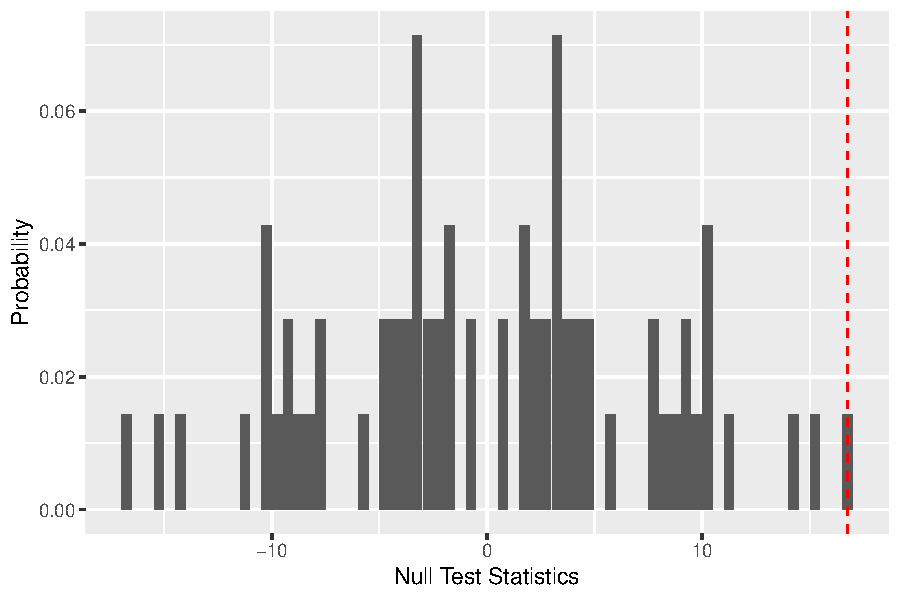
\includegraphics[width=0.9\linewidth]{null_dist_plot.pdf}
\caption{Distribution of test-stat over assignments under sharp null of no effects}
\end{figure} \vfill
\vspace{-2em}
\item Upper $p$-value is $(1/70) \approx 0.0143$
\end{itemize}  
\end{frame}
%---------------------------------------------------------------
\begin{frame}{``Lady Tasting Tea'' Example}
\vfill
\begin{itemize} \vfill
\item Upper, one-sided $p$-value \vfill
\begin{itemize} \vfill
\begin{align*}
\Pr\left(t(\bm{Z}, \bm{y}) \geq t^{\text{obs}}\right) & = \sum \limits_{\bm{z} \in \Omega} \mathbbm{1}\left\{t(\bm{z}, \bm{y}) \geq t^{\text{obs}}\right\} \Pr\left(\bm{Z} = \bm{z}\right)
\end{align*} \vfill
\end{itemize} \vfill 
\item[] \pause
\begin{align*}
\Pr\left(t(\bm{Z}, \bm{y}) \geq t^{\text{obs}}\right) & = \overbrace{\sum \limits_{\bm{z} \in \Omega}}^{\substack{\textcolor{magenta}{\text{Sum over all}} \\ \textcolor{magenta}{\text{assignments}}}} \underbrace{\mathbbm{1}\left\{t(\bm{z}, \bm{y}) \geq t^{\text{obs}}\right\}}_{\substack{\textcolor{magenta}{\text{Indicator of whether null test-stat}} \\ \textcolor{magenta}{\text{under assignment } \bm{z} \text{ is } \geq \text{ obs test-stat}}}} \underbrace{\Pr\left(\bm{Z} = \bm{z}\right)}_{\textcolor{magenta}{\text{Prob of assignment } \bm{z}}}
\end{align*} \vfill
\end{itemize} \vfill
\end{frame}
%---------------------------------------------------------------
\begin{frame}{``Lady Tasting Tea'' Example}
\vfill
\begin{itemize}
\item[]
\begin{figure}[H]
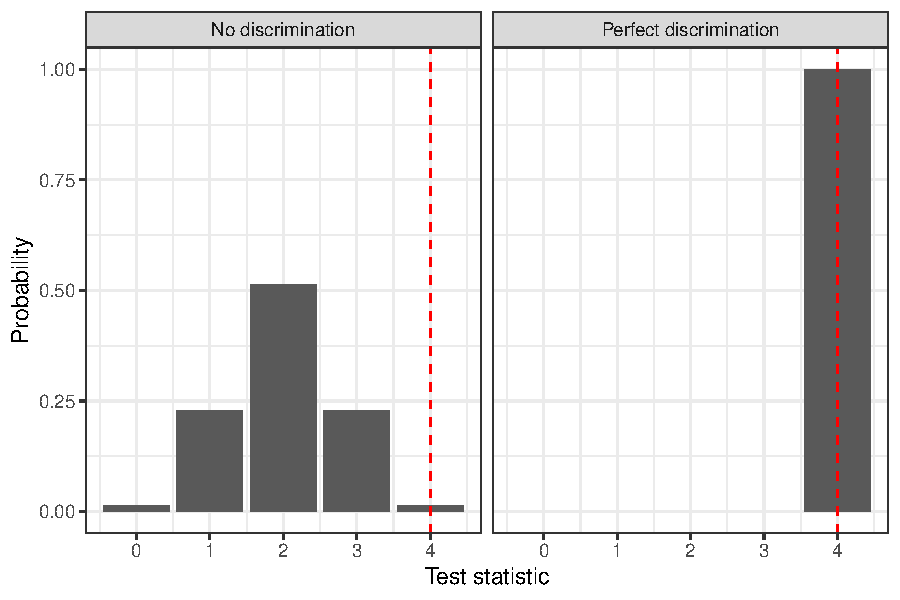
\includegraphics[width=0.9\linewidth]{perfect_discrim_test_stat_plot.pdf}
\caption{Distribution of test-stat over assignments under two sharp causal effects}
\end{figure} \vfill
\item Imagine that we test sharp null of no effects when (unbeknownst to us) true effect is that of perfect discrimination. What is power of test?
\end{itemize}  
\end{frame}
%----------------------------------------------------------------
\section{Tests of general sharp null hypotheses}
\begin{frame}{A simple model of effects for the Acorn GOTV experiment}
\vfill
\begin{itemize}
\item Consider ACORN GOTV experiment by \citet{arceneaux2005} \vfill
\item Fisher's sharp null hypothesis of no effect states that individual effect is $p = 0$ percentage points for all precincts \vfill 
\begin{table}
  \begin{tabular}{r|rr|rrr}
  \hline
 & GOTV? & vote03(\%)& $\bm{y}(\bm{0})$ & $\bm{y}(\bm{1})$ & $\bm{\tau}$\\
  \hline
1 & 0 & 38 & 38 & 38 & 0 \\
$\vdots$& & & & & \\
13 & 0 & 19 & 19 & 19 & 0 \\
14 & 0 & 34 & 34 & 34 & 0 \\
15 & 1 & 49 & 49 & 49 & 0 \\
16 & 1 & 38 & 38 & 38 & 0 \\
$\vdots$& & & & & \\
28 & 1 & 29 & 29 & 29 & 0 \\
   \hline
\end{tabular}
\end{table}
\end{itemize}  
\end{frame}
%----------------------------------------------------------------
\begin{frame}{Distribution of test-stat under sharp null of no effect}
\vfill
\begin{itemize}
\item To get a p-value, we could exactly enumerate all assignments, $\Omega$ \vfill
\item But with $\binom{28}{14} = 40,116,600$, this is too computationally intensive \vfill
\item Instead, we randomly sample from set of $\binom{28}{14}$ possible assignments \vfill
\item Then calculate test-stat under each assignment holding outcomes fixed \vfill
\begin{itemize} \vfill
\item[] E.g., Diff-in-Means $t\left(\bm{z}, \bm{y}\right) = n_T^{-1} \bm{z}^{\top}\bm{y} - n_C^{-1} \left(1 - \bm{z}\right)^{\top} \bm{y}$ \vfill
\item[] \textcolor{magenta}{{Note this test-stat is not same as one in Fisher's ``Lady Tasting Tea'', $\bm{z}^{\top}\bm{y}$}} \vfill
\end{itemize} \vfill
\item Finally, calculate p-value \vfill
\begin{equation*}
\Pr\left(t\left(\bm{Z},\bm{y}\right) \geq t^{\text{obs}}\right) = \sum \limits_{\bm{z}\in \Omega} \mathbbm{1}\left\{t\left(\bm{z}, \bm{y}\right) \geq t^{\text{obs}}\right\} \Pr\left(\bm{Z} = \bm{z}\right),
\end{equation*} \vfill
\end{itemize}  \vfill
\end{frame}
%----------------------------------------------------------------
\begin{frame}{Distribution of test-stat under sharp null of no effect}
\begin{figure}[H]
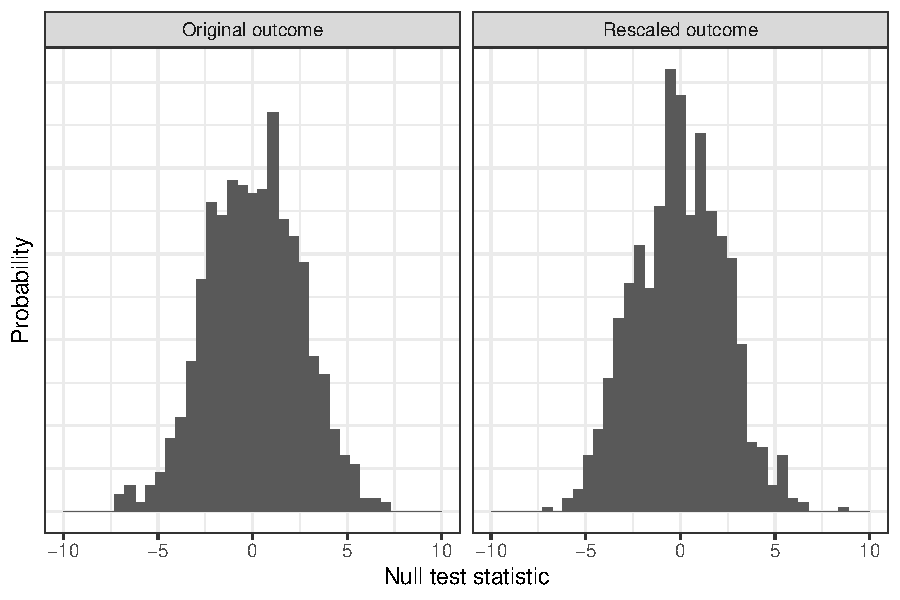
\includegraphics[width=0.9\linewidth]{null_dist_no_effect_plot.pdf}
\caption{Distribution of the Difference-in-Means test-stat under the sharp null of no effect}
\end{figure}
\end{frame}
%---------------------------------------------------------------
\begin{frame}{Hypothesis tests in adjusted outcomes}
\vfill
\begin{itemize} 
\item How do we test hypotheses other than no effect for all units? \vfill
\item \citet{rosenbaum2002a,rosenbaum2010,rosenbaum2017a}: Write units' true adjusted outcomes as $\tilde{y}_i = y_i - \tau_i z_i$ for $i = 1, \ldots , N$, where $\tau_i \coloneqq y_i(1) - y_i(0)$ \vfill
\item $\tilde{y}_i$ is fixed for every unit regardless if assigned to treatment or control
\begin{itemize} \vfill
\item I.e., $\bm{\tilde{y}} = \begin{bmatrix} \tilde{y}_1 & \tilde{y}_2 & \ldots & \tilde{y}_N \end{bmatrix}^{\top}$ satisfies sharp null of no effects \vfill
\end{itemize}
\item So to conduct a test about $\bm{\tau}$, we can compare $t(\bm{z}, \bm{\tilde{y}}_{h})$ to randomization distribution of sharp null of no effects on adjusted outcomes, $t(\bm{Z}, \bm{\tilde{y}}_{h})$, where $\tilde{y}_{hi} = y_i - z_i \tau_{hi}$ for all $i = 1, \ldots , N$ \vfill
\item \mh{Intuition}: Can we make outcomes appear as if there is no effect by removing hypothetical effect from treated units? If so, then this is evidence in favor of that hypothetical effect
\end{itemize}
\vfill
\end{frame}
%----------------------------------------------------------------
\begin{frame}{Hypothesis tests in adjusted outcomes}
\begin{itemize}
\item $H_0$: GOTV campaign increases voter turnout by $p$ percentage points per precinct  
\end{itemize}
\begin{center}
  \begin{tabular}{r|rr|rrrr}
  \hline
 & GOTV? & vote03(\%)& $\bm{\tilde{y}}_h$ & $\bm{y}(\bm{0})$ & $\bm{y}(\bm{1})$ & $\bm{\tau}$\\
  \hline
1 & 0 & 38 & 38 & 38 & ? & ?\\
$\vdots$& & & & & & \\
13 & 0 & 19 & 19 & 19& ? & ?\\
14 & 0 & 34 & 34 & 34& ? & ?\\
15 & 1 & 49 & 49 - p & ?& 49 & ?\\
16 & 1 & 38 & 38 - p & ?& 38 & ?\\
$\vdots$& & & & & & \\
28 & 1 & 29 & 29 - p & ?& 29 & ? \\
   \hline
\end{tabular}
\end{center}
\end{frame}
%----------------------------------------------------------------
\begin{frame}{Hypothesis tests in adjusted outcomes}
\begin{itemize}
\item For example, $H_0$: $p = 2.5$  
\end{itemize}
\begin{center}
  \begin{tabular}{r|rr|rrrr}
  \hline
 & GOTV? & vote03(\%)& $\bm{\tilde{y}}_h$ & $\bm{y}(\bm{0})$ & $\bm{y}(\bm{1})$ & $\bm{\tau}$\\
  \hline
1 & 0 & 38 & 38 & 38 & ? & ?\\
$\vdots$& & & & & & \\
13 & 0 & 19 & 19 & 19& ? & ?\\
14 & 0 & 34 & 34 & 34& ? & ?\\
15 & 1 & 49 & 46.5 & ?& 49 & ?\\
16 & 1 & 38 & 35.5 & ?& 38 & ?\\
$\vdots$& & & & & & \\
28 & 1 & 29 & 26.5 & ?& 29 & ? \\
   \hline
\end{tabular}
\end{center}
\begin{itemize}
\item The observed test statistic calculated on adjusted outcomes is $t(\bm{z}, \bm{\tilde{y}}_h) \approx 1.13$
\item How does it compare to $t\left(\bm{Z}, \bm{\tilde{y}}_h\right)$?
\end{itemize}
\end{frame}
%----------------------------------------------------------------
\begin{frame}{Hypothesis tests in adjusted outcomes}
\begin{figure}[H]
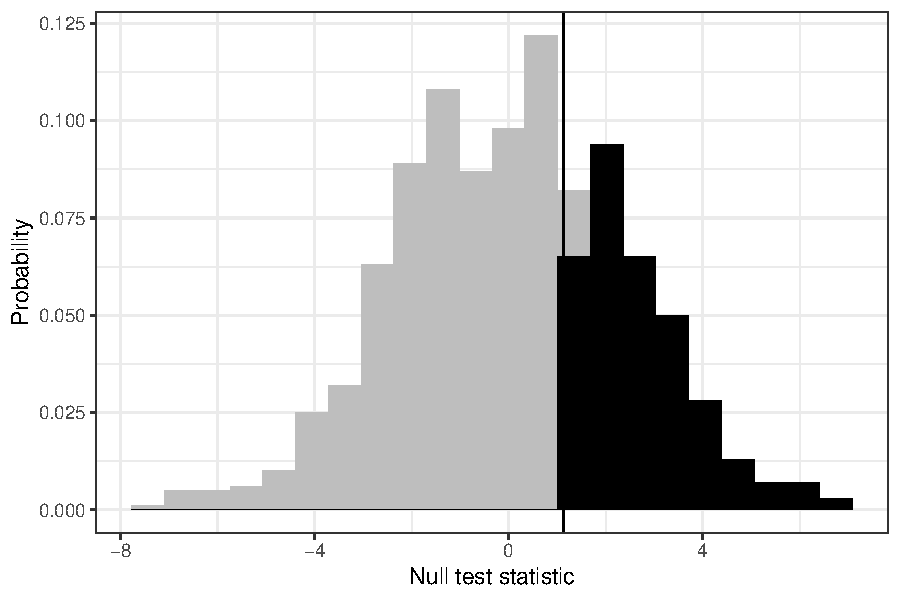
\includegraphics[width=0.9\linewidth]{null_unif_plot.pdf}
\end{figure}
\end{frame}
%----------------------------------------------------------------
\begin{frame}{Confidence sets}
\vfill
\begin{itemize} \vfill
\item To get a confidence set we do what we just did with $p = 2.5$ over an entire grid of values of $p$ \vfill
\item A $1-\alpha$ confidence set for $p$ $= $ \{$p$: $H_{p}$ not rejected at level $\alpha$\} \vfill
\item We test over all values of $p$ and retain those we fail to reject with adjusted outcomes \vfill
\item Two sided confidence set for ACORN example: $\left\{-0.4, 7.5\right\}$ \vfill
\item We fail to reject sharp null of no effect \vfill
\end{itemize}
\end{frame}
%----------------------------------------------------------------
\begin{frame}[allowframebreaks]
\frametitle{References} 
\scriptsize
\bibliographystyle{chicago}
\bibliography{Master_Bibliography}   % name your BibTeX data base
\end{frame}
%---------------------------------------------------------------











\end{document}